\section{Nástroj pro ruční přiřazení korespondujících svazků}
\label{sec:handOptim}
GUI program, který umožňuje ruční přiřazení korespondujících svazků kamene spustíme příkazem \textbf{\textit{handOptimization}}.

\subsection{Návod k obsluze}
\label{sec:snimek}

 Na začátku je zapotřebí vybrat snímek optimalizovaného kamene. Snímek vybereme v~menu \textit{File}$-$\textit{Open}$-$\textit{Image}. Po výběru snímku proběhne detekce stop v obraze a v pracovním okně se zobrazí vybraný snímek. V pracovním okně jsou na vybraný snímek zakresleny simulované svazky. Pozice vykreslení simulovaných svazků určuje transformace z \cite{Drapela}. Množina simulovaných svazků odpovídá nastavení programu. 
 
 Nastavení programu lze měnit pomocí ovládacích panelů (viz kapitola \ref{sec:panely}). V menu \textit{View} lze volit, které panely budou zobrazeny v pracovním okně.  
 
Svazky lze vykreslit třemi různými styly. Výchozí styl \textit{RadFlux} vykresluje velikost svazků podle hodnoty zářivého toku. Styl \textit{Tails} přikreslí simulované ocásky. U~stylu \textit{Polygon} je na pozici dopadu světelného svazku pomocí polygonu znázorněn tvar svazku při dopadu na stínítko, který je vůči reálným rozměrům mnohonásobně zvětšen. Vykreslené svazky lze zvětšovat či zmenšovat pomocí klávesnice $+$, resp. $-$. Styl volíme v panelu \textit{Draw setting} v kolonce \textit{Style}. 

\begin{figure}[h!]
   \centering
   \begin{minipage}[c]{0.3\textwidth}
     \centering 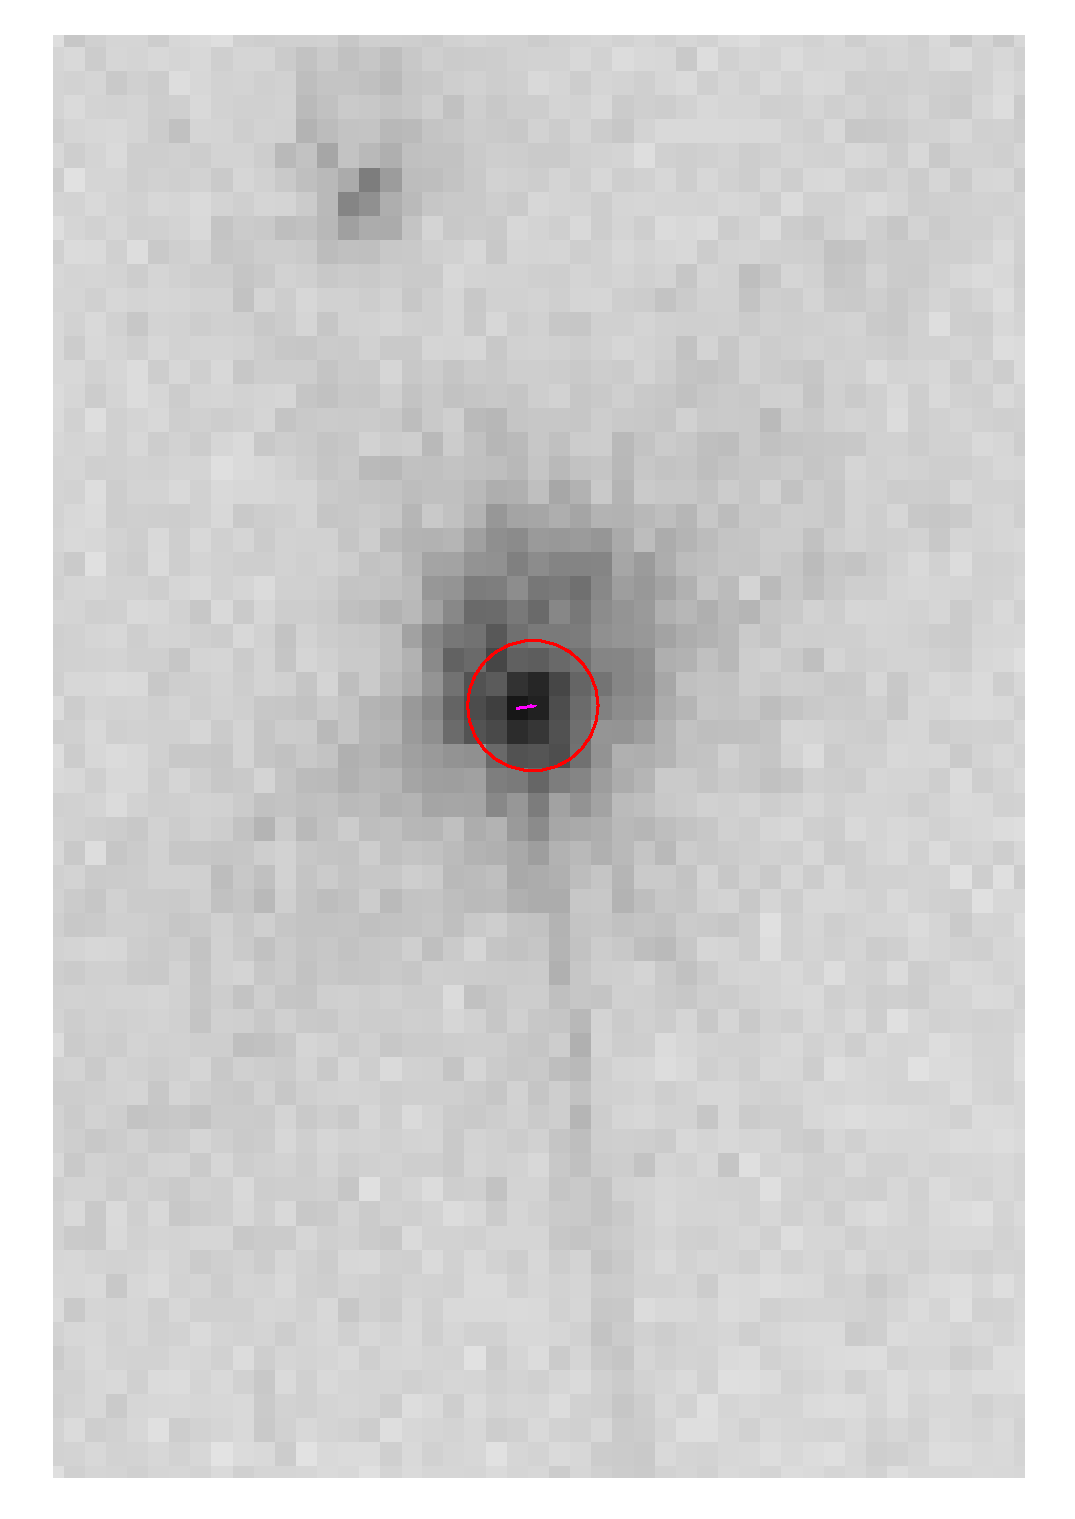
\includegraphics[width=4cm]{radFlux.pdf} 
   \end{minipage}
   \begin{minipage}[c]{0.3\textwidth}
     \centering 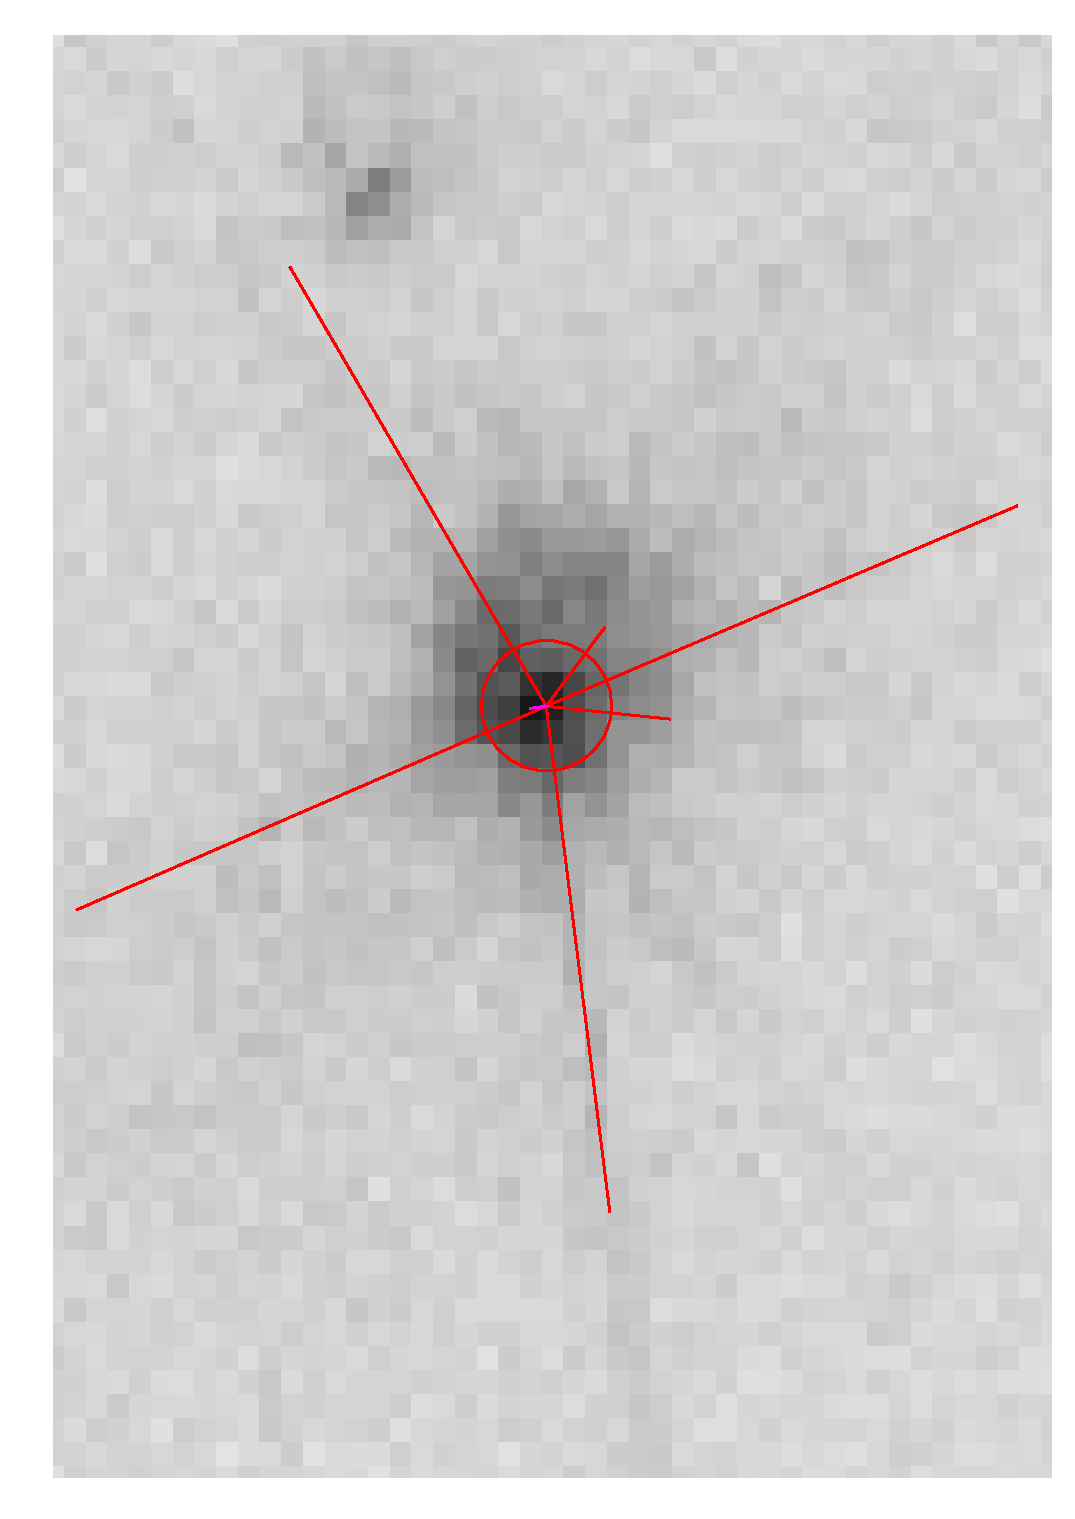
\includegraphics[width=4cm]{tails.pdf} 
   \end{minipage}
   \begin{minipage}[c]{0.3\textwidth}
     \centering 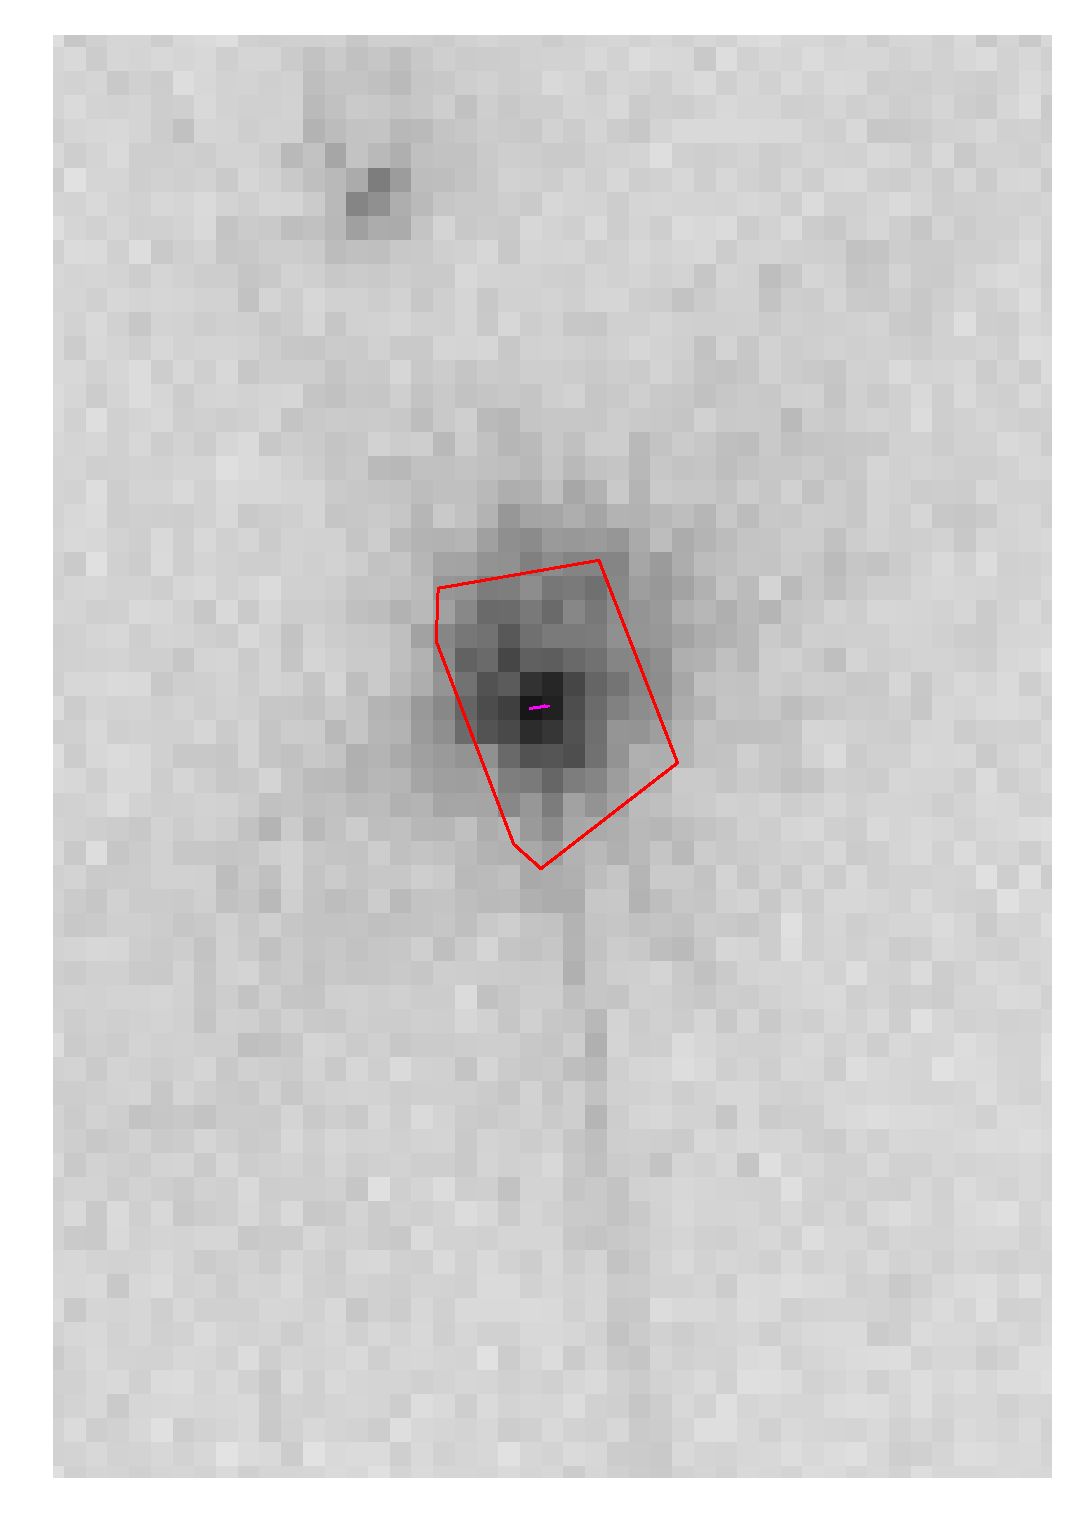
\includegraphics[width=4cm]{polygon.pdf}
   \end{minipage}
   \\
   \caption[Porovnání stylů vykreslení simulovaného svazku.]{Porovnání stylů vykreslení simulovaného svazku. Zleva \textit{RadFlux}, \textit{Tails} a \textit{Polygon}. }

\label{fig: vykresleni}
\end{figure}

 
Pokud chceme ručně přiřadit korespondující svazky, je třeba mít zvolené okénko \textit{Enable hand pairing} v panelu \textit{Correspondences}.

Pracovní okno je nastaveno tak, že reaguje na akce ovládacích prvků na optické myši. Stiskem levého tlačítka myši v oblasti snímku vybereme simulovaný svazek, který je nejblíže kurzoru myši. Po výběru svazku se zobrazí všechny detekované stopy a vybraný svazek. Opětovným stiskem levého tlačítka vybereme stopu, která spolu se svazkem utvoří korespondující pár. Po spárování se zobrazí opět pouze simulované svazky, kde jsou však barevně odděleny svazky tvořící korespondující pár. Opětovným výběrem simulovaného svazku, který již byl spárován, odstraníme odpovídající korespondující pár. 

Stiskem pravého tlačítka myši vykreslíme aktuální model kamene s vyznačenou cestou vybraného svazku.

Změnou polohy kolečka optické myši lze snímek přiblížit či oddálit, což umožňuje snadné zaměření na detaily snímku. Návrat do původního zobrazení umožňuje menu \textit{Action}$-$\textit{Reset axis}.

\begin{figure}[h!]
   \centering
   \begin{minipage}[c]{0.3\textwidth}
     \centering 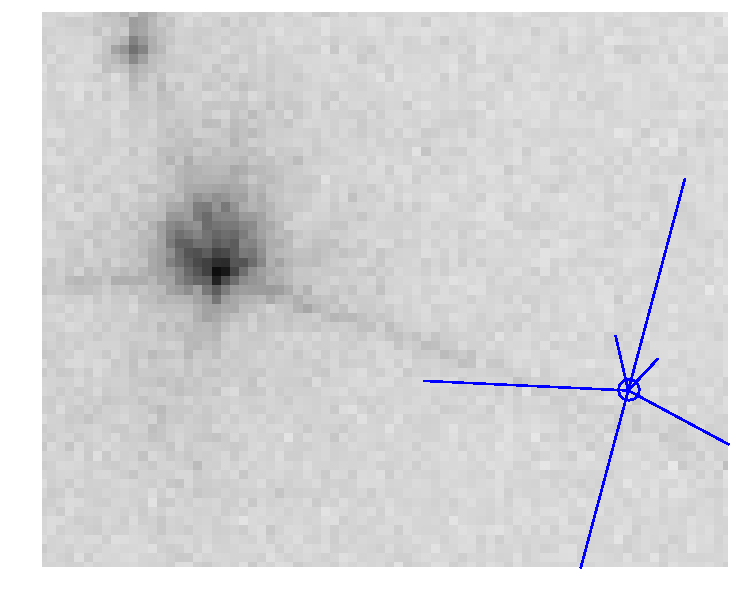
\includegraphics[width=4cm]{empty.pdf} 
   \end{minipage}
   \begin{minipage}[c]{0.3\textwidth}
     \centering 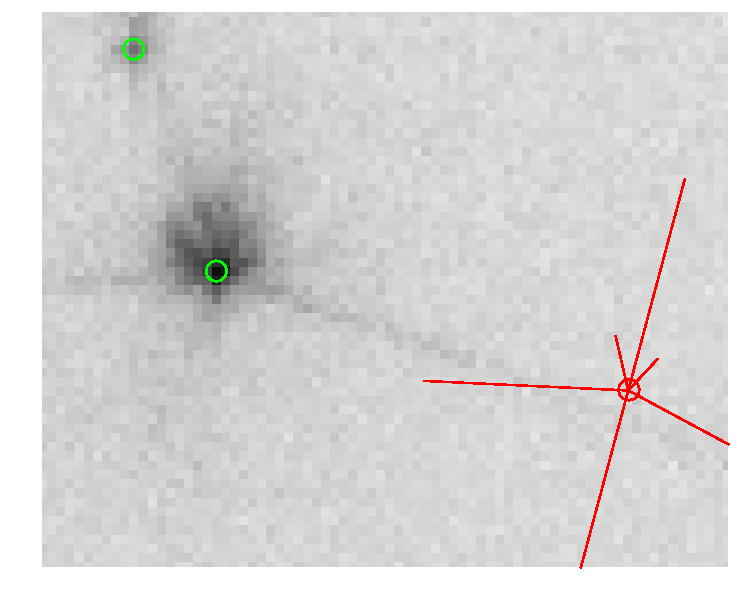
\includegraphics[width=4cm]{choosen.pdf} 
   \end{minipage}
   \begin{minipage}[c]{0.3\textwidth}
     \centering 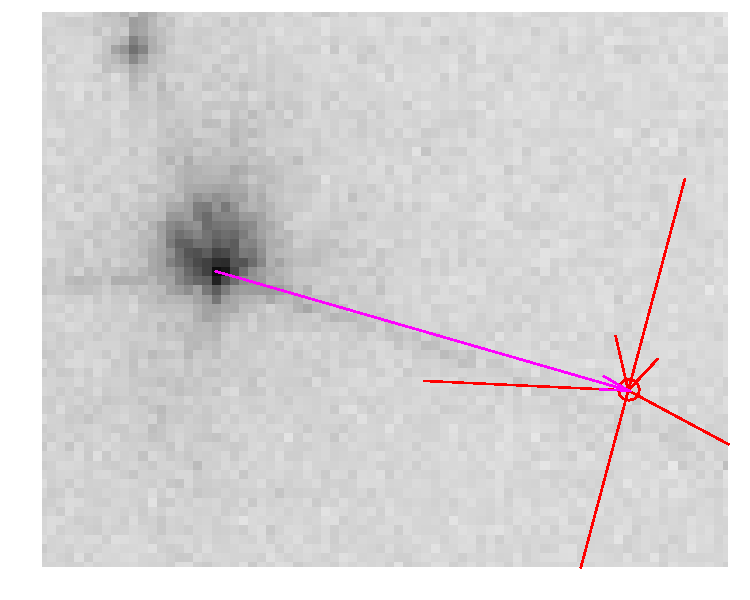
\includegraphics[width=4cm]{pair.pdf}
   \end{minipage}
   \\
   \caption[Ilustrace přiřazení simulovaného svazku ke stopě.]{Ilustrace přiřazení simulovaného svazku ke stopě. Vlevo: volný svazek. Uprostřed: vybraný svazek a zobrazené stopy. Vpravo: vytvořený pár svazek/stopa. Vykresleno stylem \textit{Tails}.}
   
\end{figure}


Soubor s množinou korespondujících svazků lze uložit v menu \textit{File}$-$\textit{Save}$-$\textit{Correspondences}. Menu \textit{File}$-$\textit{Save}$-$\textit{GUI} umožňuje uložit celé uživatelské rozhraní. 

Množinu korespondujících svazků přepíšeme, pokud načteme uložené korespondence pomocí menu \textit{File}$-$\textit{Open}$-$\textit{Correspondences}. Menu \textit{File}$-$\textit{Open}$-$\textit{Ground truth} slouží k načtení množiny správných korespondencí. Správné korespondence se porovnají s aktuální množinou korespondencí a dochází ke změně barvy, kterou jsou vykresleny simulované svazky. Zelenou barvou jsou značeny správné korespondence. Modrou barvou jsou značeny volné svazky a korespondence, u kterých nelze ověřit správnost. Červená barva náleží nesprávným korespondencím.  

V menu \textit{Action}$-$\textit{Optimize rotation} spustíme optimalizaci rotace a náklonu kamene podle korespondencí svazků třídy \textbf{1A}. Optimalizaci orientace faset spustíme v menu \textit{Action}$-$\textit{Optimize params.}. Po optimalizaci dojde k překreslení simulovaných svazků.   




%%Ovladaci panely 
%%Ovladaci panely 
%%Ovladaci panely 
%%Ovladaci panely 
\subsection{Ovládací panely}
\label{sec:panely}

\begin{wrapfigure}[14]{r}{0.3\textwidth}
\centering
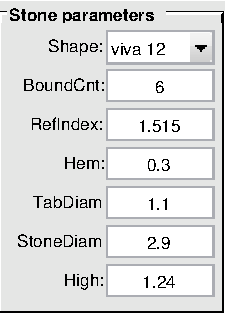
\includegraphics[width=0.3\textwidth]{StoneParameters.pdf}
	
\caption[Panel s nastavením parametrů kamene.]{Panel s nastavením parametrů kamene.}
\label{figure:stoneParameters}
\end{wrapfigure}


\paragraph{Parametry kamene}
\hspace{1mm}
\vspace{2mm}


Změřené parametry kamene (viz kapitola \ref{sec: parametryVIVA12}) lze nastavit v~panelu \textit{Stone parameters} na obrázku \ref{figure:stoneParameters}. Parametr \textit{BoundCnt} lze měnit v půběhu optimalizace. Ostatní parametry je třeba nastavit před zahájením optimalizace. Jednotky rozměrů a souřadnice jsou uváděny v milimetrech, úhly ve stupních.

\begin{itemize}
\item \textit{Shape} $-$ definuje tvar kamene. Pro tuto verzi je dostupná pouze \textit{viva12}.

\item \textit{BoundCnt} $-$ určuje maximální počet dopadových faset simulovaných svazků v programu LADOK.

\item \textit{RefIndex} $-$ index lomu kamene. Pokud je optimalizován index lomu kamene, odpovídá tato hodnota výsledku optimalizace.

\item \textit{Hem} $-$ velikost lemu kamene. 

\item \textit{TabDiam} $-$ průměr tabulky kamene. 

\item \textit{StoneDiam} $-$ průměr spodku kamene. 

\item \textit{High}	$-$ výška kamene. 
\end{itemize}

\begin{wrapfigure}[14]{r}{0.3\textwidth}
\centering
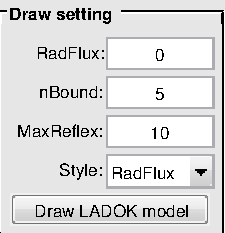
\includegraphics[width=0.3\textwidth]{DrawSetting.pdf}
	
\caption{Panel pro výběr množiny simulovaných svazků.}
\label{figure:DrawSetting}
\end{wrapfigure}

\paragraph{Zobrazení simulovaných svazků}
\hspace{1mm}
\vspace{2mm}

Panel \textit{Draw setting} na obr. \ref{figure:DrawSetting} slouží k redukci vykreslovaných simulovaných svazků. Redukce vykreslených svazků zrychlí běh programu a může pomoci v orientaci mezi jednotlivými svazky. 

\begin{itemize}
	\item  \textit{RadFlux} $-$ určuje minimální zářivý tok svazků. Vykresleny jsou simulované svazky se zářivým tokem $\phi_r$ vyšším než $\frac{\mathit{RadFlux}}{10000}$. 
	
	\item \textit{nBound} $-$ určuje počet dopadových faset vykreslených svazků. Pokud je \textit{nBound} rovno nule, jsou vykresleny všechny svazky.
	
	\item \textit{MaxReflex} $-$ omezuje vykreslení svazků na maximální počet dopadových faset \textit{MaxReflex}. 
	
	\item \textit{Style} $-$ definuje styl vykreslení simulovaných svazků. Přehled stylů je na obr. \ref{fig: vykresleni}.
	
	\item \textit{Draw LADOK model} - slouží k vykreslení aktuálního modelu kamene v programu LADOK. 
\end{itemize}


\begin{wrapfigure}[8]{r}{0.3\textwidth}
\centering
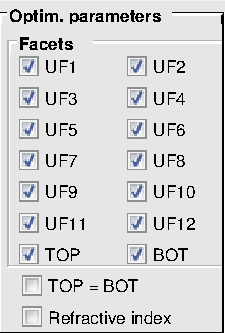
\includegraphics[width=0.3\textwidth]{OptimParameters.pdf}
	
\caption{Panel pro volbu optimalizovaných parametrů.}
\label{figure:OptimParameters}
\end{wrapfigure}

\paragraph{Optimalizované parametry}
\hspace{1mm}
\vspace{2mm}

V panelu \textit{Optim. parameters} na obr. \ref{figure:OptimParameters} můžeme volit optimalizované parametry. Mezi tyto parametry patří parametry faset a index lomu kamene. Lze vybírat jednotlivě optimalizované fasety UF1$-$UF12, TOP a BOT. Pokud zvolíme TOP$=$BOT budou parametry faset TOP a BOT během optimalizace považovány za totožné. Kolonku \textit{Refractive index} zaškrtneme, pokud chceme optimalizovat index lomu kamene. 

\newpage



\begin{wrapfigure}[16]{r}{0.3\textwidth}
\centering
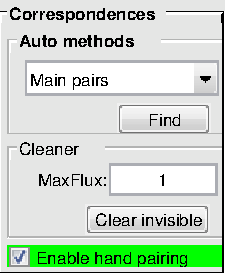
\includegraphics[width=0.3\textwidth]{Correspondences.pdf}
	
\caption{Panel pro kontrolu korespondencí svazků.}
\label{figure:Correspondences}
\end{wrapfigure}

\paragraph{Korespondence svazků}
\hspace{1mm}
\vspace{2mm}

V panelu \textit{Correspondences} na obr. \ref{figure:Correspondences} můžeme upravovat korespondence svazků. Korespondence může být přiřazena ke svazku, který odpovídá výběru v panelu \textit{Draw setting} na obr. \ref{figure:DrawSetting}.

\begin{itemize}
	\item \textit{Auto methods} $-$ obsahuje automatické metody pro určení korespondujících svazků. \textit{Main pairs} nalezne korespondence tříd \textbf{1A}, \textbf{3A} a \textbf{5D}. \textit{Tails} nalezne korespondence svazků podle algoritmu \ref{sec: korespondence_ocasky}. \textit{RadFlux} určí korespondující svazky na základě algoritmu \ref{sec: poloha_tok}.  
	
	\item \textit{Cleaner} $-$ slouží k odstranění korespondencí, které jsou z vysoké pravděpodobnosti nesprávné. Po vyplnění pole \textit{MaxFlux} jsou odstraněny všechny korespondence, kde simulovaný svazek má zářivý tok nižší než $\frac{\mathit{MaxFlux}}{10000}$. \textit{Clear invisible} odstraní korespondence, pro které simulovaný svazek v aktuálním modelu neexistuje. 
	
	\item \textit{Enable hand pairing} $-$ povolí ruční korespondenci simulovaných a pozorovaných svazků.
\end{itemize}


\begin{wrapfigure}[5]{r}{0.3\textwidth}
\centering
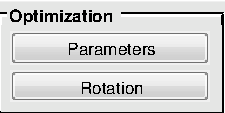
\includegraphics[width=0.3\textwidth]{Optimization.pdf}
	
\caption{Panel pro výběr optimalizační úlohy. }
\label{figure:Optimization}
\end{wrapfigure}


\paragraph{Optimalizace}
\hspace{1mm}
\vspace{2mm}

Panel \textit{Optimization} na obr. \ref{figure:Optimization} slouží k volbě optimalizační úlohy.
 
\begin{itemize}
	\item \textit{Parameters} $-$ optimalizují se parametry faset podle výběru v panelu \textit{Optim. parameters} na obr. \ref{figure:OptimParameters}.
	
	\item \textit{Rotation} $-$ optimalizuje se rotace a sklon kamene. 
\end{itemize}


\begin{wrapfigure}[5]{r}{0.3\textwidth}
\centering
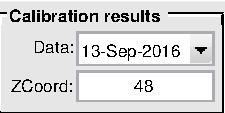
\includegraphics[width=0.3\textwidth]{CalibrationResults.pdf}
	
\caption{Panel pro volbu výsledků kalibrace. }
\label{figure:CalibrationResults}
\end{wrapfigure}

\paragraph{Výsledky kalibrace}
\hspace{1mm}
\vspace{2mm}

Panel \textit{Calibration results} na obr. \ref{figure:CalibrationResults} slouží k načtení výsledků kalibrace. 
 
\begin{itemize}
	\item \textit{Data} $-$ výsledek kalibrace podle data. Soubory s výsledky kalibrace jsou v určeném adresáři. 
	
	\item \textit{ZCoord} $-$ upraví $z$ souřadnici kamene. 
\end{itemize}


\newpage

\begin{wrapfigure}[6]{r}{0.3\textwidth}
\centering
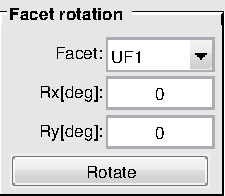
\includegraphics[width=0.3\textwidth]{FacetRotation.pdf}
	
\caption{Panel pro změnu sklonu normál faset. }
\label{figure:FacetRotation}
\end{wrapfigure}

\paragraph{Rotace faset}
\hspace{1mm}
\vspace{2mm}

Panel \textit{Facet rotation} na obr. \ref{figure:FacetRotation} slouží k rotaci vybrané fasety. Fasetu vybereme v nabídce \textit{Facet}, zadáme úhel rotace \textit{$R_x$} v ose $x$ a \textit{$R_y$} v ose $y$. Stiskem \textit{Rotation} natočíme vybranou fasetu o~zvolený úhel. Po rotaci kamene se přepočítají simulované svazky.  
 
 \vspace{3cm}

\paragraph{Parametry faset}
\hspace{1mm}
\vspace{2mm}

Panel \textit{Facet parameters} na obr. \ref{figure:FacetParameters} slouží ke zobrazení výsledků optimalizace. Parametr $\alpha_{ref}$ označuje azimut počátečního dohadu normály fasety. Parametr $\Delta\alpha$ ukazuje změnu azimutu optimalizovaného modelu vůči původnímu odhadu. Podobně pro elevaci  $\varepsilon$. Uvedené výsledky jsou v úhlových stupních. 
 
\begin{figure}[h!]
\centering
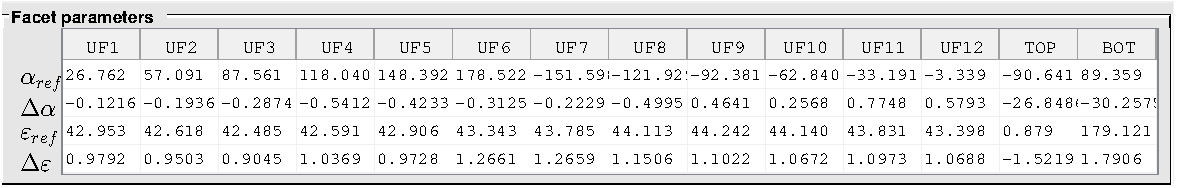
\includegraphics[width=\textwidth]{FacetParameters.pdf}
	
\caption{Panel pro zobrazení výsledků optimalizace.}
\label{figure:FacetParameters}
\end{figure}
 


  
\clearpage